\documentclass[conference]{report}
\usepackage{graphicx}  % Allows inclusion of images
\usepackage{listings}  % Code formatting
\usepackage{xcolor}    % Colors for code highlighting
\usepackage{hyperref}  % Hyperlinks in the document
\usepackage{tikz}
\usepackage{url}
\usepackage{graphicx}
%Includes "References" in the table of contents
\usepackage[nottoc]{tocbibind}
\usetikzlibrary{shapes, arrows, positioning}
% Define Rust syntax highlighting

\lstdefinelanguage{Rust}{
morekeywords={fn, let, mut, move, loop, match, if, else, while, for, break, continue, return, struct, impl, pub, use, mod, crate, super, Self, as, const, static, ref, trait, enum, type, where, unsafe, async, await},
sensitive=true,
morecomment=[l]{//},
morecomment=[s]{/}{/},
morestring=[b]"
}

\lstset{
language=Rust,
basicstyle=\ttfamily\footnotesize,
keywordstyle=\color{blue},
commentstyle=\color{green!70!black},
stringstyle=\color{orange},
numbers=left,
numberstyle=\tiny\color{gray},
stepnumber=1,
showstringspaces=false,
breaklines=true,
frame=single,
captionpos=b
}

\nocite{*} % This command ensures that all entries in myBib.bib are included

\bibliographystyle{acm}

\begin{document}

\title{Multi-Threaded Programming
and IPC in Rust}
\author{James Morelli \\ \small NetId: 3502 \\ \small Operating Systems}
\date{\today}

\maketitle
\tableofcontents
\chapter{Introduction}
This project will cover the implementation of multi-threading and inter-process communication (IPC) using the Rust programming language. It aims to use these fundamental operating systems functionality to create mock banking scenario where multiple customers can request bank transfers. All of these transfers should happen concurrently and demonstrate safe data access in a multi threaded environment. 
\section*{Objectives and Scope}

\subsection*{Objectives}
The primary objectives of this project are:
\begin{itemize}
    \item Develop and implement a robust multi-threaded system.
    \item Ensure safe concurrent data access using mutexes and atomic operations.
    \item Facilitate inter-process communication via named pipes.
    \item Integrate these components into a comprehensive, mock banking scenario.
\end{itemize}

\subsection*{Scope}
This project focuses on demonstrating key operating system concepts and concurrent programming techniques in Rust. The scope includes:
\begin{itemize}
    \item \textbf{Multi-threading:} Design and implementation of a system that spawns multiple threads to simulate concurrent bank transactions.
    \item \textbf{Synchronization:} Utilization of synchronization primitives such as mutexes and atomic types to safely manage shared data across threads.
    \item \textbf{Inter-Process Communication (IPC):} Implementation of IPC using named pipes (FIFOs) to allow communication between separate processes, simulating distributed components of the banking system.
    \item \textbf{System Integration:} Combining the multi-threading and IPC components into a fully functional mock bank application, where multiple customers can request transfers concurrently.
\end{itemize}

\section*{Approach}
The approach for this program was to build each phase in sequence. Dividing each progression into different files to track changes and enhancements to meet each new requirement. This allowed for better understanding of exactly what was being expanded ie. thread management to mutex locks for consistent and safe data access from phase 1 to 2. Once each phase for thread management and IPC requirements were completed I endeavored to integrate each section for a wholistic design and utilization of Rust. Initially I kept each file isolated for ease of reading and understanding but with the integration I wanted this design to be more true to what a fully functioning program would be structured using best practices.

\chapter{Implementation Details}

This chapter describes the step-by-step development of the system's core components—multi-threading and inter-process communication (IPC)—and their subsequent integration into a unified mock banking application.

\section*{Threading Solution}
The threading solution was developed incrementally over several phases:

\subsection*{Phase 1: Basic Thread Simulation}
Initially, simple threads were created to simulate transactions. Each thread waited for a random duration and printed log messages to mimic a bank transaction.

\subsection*{Phase 2: Shared Account Access}
In this phase, we introduced safe concurrent data access by wrapping an \texttt{Account} structure in an \texttt{Arc<Mutex<Account>>}. This allowed multiple threads to access and modify the account data without causing race conditions.

\hfill
\begin{lstlisting}[caption={Creating a Thread-Accessible Account}, label=code:phase2-account-creation]
let account = Arc::new(Mutex::new(Account { balance: 1000 }));

...

// Acquire the account lock.
let mut account_lock = account_clone.lock().unwrap();
account_lock.balance += random_deposit;
\end{lstlisting}

The use of a mutex ensures that only one thread can modify the account at a time. In Rust, the lock is automatically released when its guard goes out of scope, thereby allowing other threads to access the data safely.

\subsection*{Phase 3: Exploring Deadlocks}
To better understand deadlock conditions, Phase 3 involved intentionally creating deadlocks. Instead of a single account, two separate accounts were used for fund transfers. When transferring funds in one direction (e.g., Account 1 to Account 2), locks were acquired in a consistent order, so no deadlock occurred. However, when transfers were initiated in both directions simultaneously, each thread attempted to lock the accounts in a different order, leading to a deadlock.

\hfill
\begin{lstlisting}[caption={Deadlock Creation Example}, label=code:phase3-deadlock]
let transaction1 = transfer(
    Arc::clone(&account1),
    Arc::clone(&account2),
    format!("{}", thread_id),
    TransactionAction::Deposit
);
let transaction2 = transfer(
    Arc::clone(&account1),
    Arc::clone(&account2),
    format!("{}-2", thread_id),
    TransactionAction::Withdraw
);
\end{lstlisting}

To address this, deadlock detection was implemented using a loop that monitored the duration of the lock acquisition attempt. By using the non-blocking \texttt{try\_lock} method for the second account, the system can detect potential deadlocks and respond accordingly.

\hfill
\begin{lstlisting}[caption={Deadlock Detection Example}, label=code:phase3-detection]
while transaction_start.elapsed() < Duration::from_millis(1000) {
    // Acquire lock on the source account (blocking).
    let from_lock = from.lock();
    // Attempt to acquire lock on the destination account (non-blocking).
    let to_lock = to.try_lock();
    ...
}
\end{lstlisting}

\subsection*{Phase 4: Deadlock Prevention}
In Phase 4, the transfer function was refined to enforce a consistent lock acquisition order. By abstracting the order of the accounts from the direction of the fund transfer and introducing a \texttt{TransactionAction} enum, the system now determines the proper order to lock the accounts, thus preventing deadlocks during concurrent transfers.

\section*{Inter-Process Communication}
The IPC component was implemented using a named pipe (FIFO) to facilitate communication between separate processes. In the \texttt{ipc.rs} binary, a producer process writes messages to the FIFO file, and a consumer process reads from it. The consumer then transforms the message and logs the output to the console.

\hfill
\begin{lstlisting}[caption={Creating Multiple Processes}, label=code:ipc-start]
let producer_thread = thread::spawn(move || {
    let mut producer = Command::new("cargo")
        .arg("run")
        .arg("--bin")
        .arg("producer")
        .arg(producer_file_full_path)
        .spawn()
        .expect("Failed to start producer");

    producer.wait().expect("Producer process failed");
});

// Create a consumer process.
let mut consumer = Command::new("cargo")
    .arg("run")
    .arg("--bin")
    .arg("consumer")
    .spawn()
    .expect("Failed to start consumer");
\end{lstlisting}

Several challenges arose during the IPC implementation. For example, the FIFO file needed to be properly created and deleted on each run. Additionally, when multiple producer processes attempted concurrent writes, their outputs occasionally intermingled. A temporary fix limited the system to a single producer, though a more robust solution was implemented during full integration.

\section*{Integration}
The final phase integrated the multi-threading and IPC components into a cohesive system that more accurately reflects a realistic banking scenario. In the integrated system:
\begin{itemize}
    \item \textbf{Customer Processes:} Run as separate processes, where each customer sends a transfer request through the named pipe.
    \item \textbf{Bank Teller Process:} Acts as a consumer that reads incoming requests, determines the appropriate accounts, and initiates fund transfers.
    \item \textbf{Concurrent Transfer Processing:} Each transfer is handled in a separate thread, ensuring that the teller can continue processing incoming requests without delay.
\end{itemize}

A high-level diagram (see Figure~\ref{fig:integration-flow}) illustrates the overall system architecture, including the interplay between processes, threads, and the IPC mechanism.

\hfill

\begin{figure}[h]
    \centering
    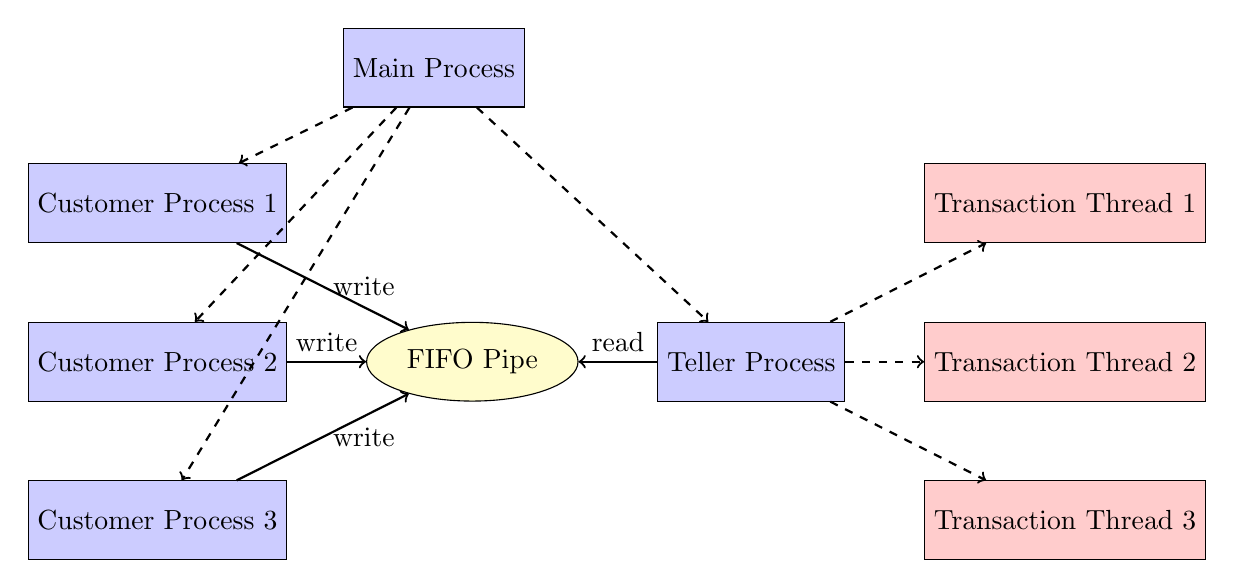
\begin{tikzpicture}[
    node distance=1cm, auto,
    process/.style={rectangle, draw, fill=blue!20, minimum size=1cm},
    thread/.style={rectangle, draw, fill=red!20, minimum size=1cm},
    ipc/.style={ellipse, draw, fill=yellow!20, minimum size=1cm},
    arrow/.style={->, thick}
    ]

    % Main process node
    \node (main) [process] {Main Process};

    % Customer processes nodes
    \node (customer1) [process, below left=of main] {Customer Process 1};
    \node (customer2) [process, below=of customer1] {Customer Process 2};
    \node (customer3) [process, below=of customer2] {Customer Process 3};
    
    % IPC FIFO pipe node
    \node (fifo) [ipc, right=of customer2] {FIFO Pipe};

    % Teller process node
    \node (teller) [process, right=of fifo] {Teller Process};

    % Transaction Thread Nodes
    \node (thread2) [thread, right=of teller] {Transaction Thread 2};
    \node (thread1) [thread, above=of thread2] {Transaction Thread 1};
    \node (thread3) [thread, below=of thread2] {Transaction Thread 3};

    % Arrows indicating communication channels
    \draw[arrow] (customer1) -- (fifo) node[midway, right] {write};
    \draw[arrow] (customer2) -- (fifo) node[midway, above] {write};
    \draw[arrow] (customer3) -- (fifo) node[midway, right] {write};
    \draw[arrow] (teller) -- (fifo) node[midway, above] {read};

    % Arrows showing spawning relationships
    \draw[arrow, dashed] (main) -- (customer1);
    \draw[arrow, dashed] (main) -- (customer2);
    \draw[arrow, dashed] (main) -- (customer3);
    \draw[arrow, dashed] (main) -- (teller);
    \draw[arrow, dashed] (teller) -- (thread1);
    \draw[arrow, dashed] (teller) -- (thread2);
    \draw[arrow, dashed] (teller) -- (thread3);
\end{tikzpicture}

    \caption{Integration Process and Thread Flow}
    \label{fig:integration-flow}
\end{figure}

\subsection*{Integration Improvements}
During the integration phase, several key enhancements were implemented to ensure that all components work cohesively:

\begin{itemize}
    \item \textbf{Logical Separation of Classes and Functionality:} The project was refactored to clearly delineate class responsibilities and functionality. This reorganization not only mirrors real-world software design but also significantly improves code clarity and readability.
    \item \textbf{File Locking with \texttt{nix}:} A third-party library, \texttt{nix}, was integrated to allow threads to lock the file. This enhancement addresses the IPC issue where multiple producers were writing messages on the same line.
    \item \textbf{Fine-Grained Mutex Usage:} The \texttt{Mutex} was moved into the account class to specifically protect the \texttt{balance} attribute. This ensures that only the relevant property is locked during operations, thereby reducing contention and improving concurrent performance.
\end{itemize}

\chapter{Environment Setup}
This section details the process of setting up Ubuntu on my personal device. To establish a functional development environment, I installed Ubuntu on a secondary drive in an older Acer laptop. This approach provided a quick and efficient setup while significantly outperforming previous attempts using a virtual machine in terms of speed and responsiveness.  

Moving forward, I plan to keep Ubuntu installed on this device for personal development and testing. I find the Linux operating system to be highly intuitive, and I prefer the Bash shell over Windows PowerShell due to its streamlined syntax and greater flexibility for scripting and automation.

\section*{Tools Used}
The programming language selected for this project was Rust. Initially, I found Rust challenging, particularly due to its ownership rules. However, its strict compile-time checks provided immediate feedback, preventing mistakes from propagating too far. Even small sections of code would quickly trigger compiler errors, which significantly accelerated my learning process and improved my understanding of ownership and borrowing concepts.  

One of the most rewarding aspects of learning Rust was experiencing a programming language without a garbage collector for the first time. This required me to be more mindful of memory management and avoid unnecessary object copying. As a result, I gained a deeper understanding of efficient resource allocation and memory optimization. Additionally, this experience has enhanced my comprehension of the singleton model in Java, particularly in terms of managing object lifetimes and reducing redundant allocations.

\section*{Challenges}
The development environment initially was attempted with a VM on an M2 Mac device; this was tried with VirtualBox and UTM. I had a lot of trouble with this configuration as the VM software would start and install Ubuntu on the VM but when it would restart the entire system would refresh and restart the install. I believe this had to do with how the VM was attempting to partition my drives. I solved this by creating a boot-able USB drive with Ubuntu (used Rufus to create the drive) and dual-loaded this onto a Windows machine.

\chapter{Challenges and Solutions}

This project presented some interesting challenges that helped me better understand how Rust manages data and handles multiple tasks at the same time.

\subsection*{Rust Ownership and Cloning}
One of the primary challenges was adapting to Rust's ownership model. It took time to understand when to clone an object versus when to use a reference. This learning curve was critical to ensure that data could be safely shared across threads.

\subsection*{Deadlock Management}
Managing deadlocks was another significant challenge. Setting up controlled deadlock scenarios helped in understanding their causes and how to handle them gracefully. In the integration phase, determining the correct order of locking accounts and assigning appropriate wait times was essential, especially when the sequence of account access was unpredictable.

\subsection*{Debugging and Testing}
Initially, I relied on CodeLLDB, a debugger for Rust, to step through the code. However, as the project evolved to include multiple processes and threads, the debuggers usefulness fell off. Instead, unit tests for individual methods became a crucial tool for verifying functionality and diagnosing issues.

\subsection*{Leveraging External Resources}
The comprehensive guides available on the official Rust website greatly expanded my understanding of Rust’s intricacies. Additionally, ChatGPT proved to be a valuable resource for troubleshooting, researching solutions, and identifying useful third-party libraries to address specific problems.

\chapter{Results and Outcomes}

\subsection{Summary}

The integration of multi-threading and inter-process communication has produced a system capable of handling multiple customers and processing transactions across 10 accounts concurrently. The program efficiently processes transactions by employing a fallback mechanism for deadlock resolution, ensuring that all required locks are eventually acquired. Communication is managed through a named pipe, resulting in race-free and safely managed operations.

\subsection{Metrics and Testing}

Performance benchmarks and unit tests confirmed that the system reliably handles concurrent requests and resolves deadlocks within acceptable time limits. See Figure~\ref{fig:perf-1} for the benchmark times when there are random transaction delays to add fake processing time.

\begin{figure}[ht]
    \centering
    \includegraphics[width=0.5\linewidth]{perf-1.png}
    \caption{Perf Report with Transaction Delay}
    \label{fig:perf-1}
\end{figure}

When the delays are removed from the program we can see the transaction processing which was taking up most of the time in the program drops completely off of the top overhead figures.

\begin{figure}[ht]
    \centering
    \includegraphics[width=0.5\linewidth]{perf-2.png}
    \caption{Perf Report without Transaction Delay}
    \label{fig:perf-2}
\end{figure}

\subsection{Limitations}

Despite its successes, the system has several limitations that suggest directions for future improvements. A major limitation is the use of a small, static dataset of only 10 accounts. Employing a database with a larger selection of accounts and more complex transaction criteria would better demonstrate the scalability and real-world applicability of the system. Additionally, while the current deadlock resolution strategy works under moderate loads, it may not scale effectively; preliminary tests indicate that with more than 50 concurrent requests, deadlocks could lead to dropped transactions. Further enhancements in deadlock detection and resolution mechanisms are recommended to improve performance under higher demand.

\chapter{Reflection and Learning}

This project helped me learn a lot about Rust and its unique approach to memory management and system-level programming. It made me realize how much I had taken for granted the conveniences of garbage-collected languages, emphasizing the need for careful resource handling. I gained a deeper understanding of operating systems and threading, along with the challenges posed by concurrency. Additionally, exploring inter-process communication via pipes offered a new perspective on the inner workings of Bash scripting and system commands.

\bibliography{myBib}

\end{document}